\subsection{M-twisted differential forms}

10.3.1. Let X be a real manifold of class \(C^{r}\) and let M be a vector bundle with base X, of finite rank and of class \(C^{k}\), with \(0 \leqslant k \leqslant r\). Let \(\lambda_{\mathrm{M}} = (\mathrm{Or}_{\mathrm{M}}, \{\pm 1\}, \mathrm{X}, \pi)\) be the principal fibration associated with the manifold of orientations of M (10.2.2). Let the structural group \(\{\pm 1\}\) act on R by multiplication. We denote by \(\tilde{R}_{M}\) the bundle associated with \(\lambda_{M}\) of fiber type R (endowed with the operation law defined above) (6.5.1); it is equipped (7.10.2) with a vector bundle structure over the base X, of rank 1 and class \(C^{k}\); it is called the bundle of M-twisted scalars.

10.3.2. We have a commutative diagram:

\pandocbounded{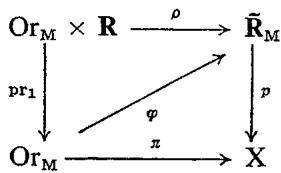
\includegraphics[keepaspectratio]{images/part001_9c73fb1b.jpg}}

where \(p\) denotes the canonical projection of \(\tilde{\mathbf{R}}_{\mathbf{M}}\) onto \(\mathbf{X}\), \(\rho\) the frame map (6.5.1) of \(\tilde{\mathbf{R}}_{\mathbf{M}}\), and where \(\varphi(\xi) = \rho(\xi, 1)\) for \(\xi \in \mathrm{Or}_{\mathbf{M}}\). In particular, the inverse image of the bundle \(\tilde{\mathbf{R}}_{\mathbf{M}}\) by \(\pi\) is identified with the trivial bundle \(\mathrm{Or}_{\mathbf{M}} \times \mathbf{R}\). One also identifies an element \(\xi\) of \(\mathrm{Or}_{\mathbf{M}}\) with its image in \(\tilde{\mathbf{R}}_{\mathbf{M}}\) by \(\varphi\); with this convention, one has \(\rho(\xi, a) = a\xi\) for all \((\xi, a) \in \mathrm{Or}_{\mathbf{M}} \times \mathbf{R}\); we have \(a\xi = b\eta\) if and only if there exists \(e \in \{\pm 1\}\) such that \(b = ea\) and \(\eta = e\xi\). An orientation \(\xi\) of \(\mathbf{M}\) thus defines a section \(x \mapsto \xi(x)\) of \(\tilde{\mathbf{R}}_{\mathbf{M}}\).

There exists one and only one isomorphism \(j\) from \(\tilde{\mathbf{R}}_{\mathbf{M}} \otimes \tilde{\mathbf{R}}_{\mathbf{M}}\) onto the trivial bundle \(\mathbf{R}_{\mathbf{x}} = \mathbf{X} \times \mathbf{R}\) such that \(j(\xi \otimes \xi) = (\pi(\xi), 1)\) for all \(\xi \in \mathrm{Or}_{\mathbf{M}}\); this allows one to identify the vector bundle \(\tilde{\mathbf{R}}_{\mathbf{M}}\) with its dual.

10.3.3. Let F moreover be a vector bundle over the base X and of class \(C^{r-1}\). A differential form on X with values in \(\tilde{R}_{M} \otimes F\) is called an M-twisted differential form with values in F. Such a form of degree p is a section of the bundle \(\operatorname{Alt}^{p}(\mathrm{T}(\mathrm{X}); \tilde{\mathbf{R}}_{\mathbf{M}} \otimes \mathbf{F})\), which one identifies in the obvious way with \(\tilde{R}_{M} \otimes \operatorname{Alt}^{p}(\mathrm{T}(\mathrm{X}); \mathbf{F})\). When F is the trivial bundle defined by a Banach space E, one speaks simply of an M-twisted form with values in E; when E = C (resp. R), one says complex M-twisted form (resp. real M-twisted form, or M-twisted form).

Let \(\omega\) be an M-twisted form of degree \(p\) with values in F. The fact that \(\pi\colon\mathrm{Or}_{\mathbb{M}}\to\mathbf{X}\) is étale and that \(\pi^{*}(\tilde{\mathbf{R}}_{\mathbb{M}})=\mathrm{Or}_{\mathbb{M}}\times\mathbf{R}\) allows one to identify \(\pi^{*}(\tilde{\mathbf{R}}_{\mathbb{M}}\otimes\operatorname{Alt}^{p}(\mathrm{T}(\mathrm{X});\mathrm{F}))\) with \(\mathrm{Alt}^{p}(\mathrm{T}(\mathrm{Or}_{\mathbb{M}});\pi^{*}(\mathrm{F}))\), and \(\omega\) defines a section \(\tilde{\omega}\) of \(\mathrm{Alt}^{p}(\mathrm{T}(\mathrm{Or}_{\mathbb{M}});\pi^{*}(\mathrm{F}))\) (7.4.3), in other words, a differential form of degree \(p\) on \(\mathrm{Or}_{\mathbb{M}}\) with values in \(\pi^{*}(\mathrm{F})\). This yields a bijection from the space of M-twisted forms of degree \(p\) on X with values in F onto the space of forms \(\tilde{\omega}\) of degree \(p\) on \(\mathrm{Or}_{\mathbb{M}}\) with values in \(\pi^{*}(\mathrm{F})\) such that

\[
\tilde{\omega}(-\xi)=-\tilde{\omega}(\xi)\quad\text{for every }\xi\in\mathrm{Or}_{\mathbb{M}}.
\]

When M is equipped with an orientation \(\xi\), the map \(\omega \mapsto \xi \otimes \omega\) makes it possible to identify the sections of \(\mathrm{Alt}^p(\mathrm{T}(\mathrm{X});\mathrm{F})\) (in other words, the usual differential forms of degree \(p\)) with M-twisted forms of degree \(p\) with values in F.

10.3.4. Let \(\omega\) be an M-twisted differential form of degree \(p\) on X, with values in a Banach space E, and of class \(\mathbf{C}^s\) (\(1 \leqslant s \leqslant \inf(k, r - 1)\)). There exists one and only one M-twisted differential form \(d\omega\), of degree \(p + 1\) on X, with values in E, such that, for every open set U of X, every orientation \(\xi\) of \(M|_{U}\), and every differential form \(\alpha\) on U such that \(\omega|_{U} = \xi \otimes \alpha\), one has \(d\omega|_{U} = \xi \otimes d\alpha\). The form \(d\omega\) is of class \(\mathbf{C}^{s-1}\); it is called the exterior differential of \(\omega\).

If one denotes by \(\tilde{\omega}\) (resp. \(\widetilde{d\omega}\)) the differential form on \(\mathrm{Or}_{\mathbb{M}}\) corresponding to \(\omega\) (respectively to \(d\omega\)) as in 10.3.3, one has \(d(\tilde{\omega}) = \widetilde{d\omega}\).

If \(\zeta\) is a vector field of class \(\mathbf{C}^s\) onto \(X\) , one defines in an analogous manner the M-twisted form \(\theta_{\zeta}.\omega\) . One has

\[
\theta_ {\zeta}. \omega = d (i (\zeta) \omega) + i (\zeta) d \omega
\]

and \(\theta_{\zeta}.\omega\) is of class \(\mathbf{C}^{s - 1}\).

